\documentclass[a4paper,hidelinks,14pt]{extarticle}

\usepackage[utf8]{inputenc}
\usepackage[T2A]{fontenc}
\usepackage[english, russian]{babel}
\usepackage{amsmath}
\usepackage{amsfonts}
\usepackage{mathtools}
\usepackage{datetime}
\usepackage[pdftex]{graphicx}
\usepackage{indentfirst}
\usepackage{asymptote}
\usepackage{systeme}
\usepackage{listings}
\usepackage[usenames,dvipsnames]{color}	
\usepackage[framed,autolinebreaks,useliterate]{mcode}
\usepackage[font={small,it}]{caption}
	
\begin{document}
	\begin{titlepage}
		\setlength{\parindent}{0ex}
		
		\begin{center}
			\textsc{
				\vspace{1ex}
				Научно исследовательский университет ИТМО \\
				\vspace{0.5ex}
				Факультет систем управления и робототехники \\
				\vspace{0.5ex}
			}
		\end{center}
		
		\vspace{50mm}
		
		\begin{center}
			Отчет по лабораторной работе №6 \\
			Сжатие изображений
		\end{center}
		
		\vspace{50mm}
		
		\begin{minipage}{.55\linewidth}
			Выполнил студент группы R3280
			
			\smallskip
			
			Преподаватель
		\end{minipage}
		\hfill
		\begin{minipage}{.4\linewidth}
			\begin{flushright}
				Мовчан И. Е.
				\\
				Перегудин А. А.
			\end{flushright}
		\end{minipage}
		
		\vfill
		\begin{center}
			Санкт-Петербург
			\\
			2024
		\end{center}
		
	\end{titlepage}
	
	\subsection*{Выбор изображения и его обработка}
	Будем обрабатывать и исследовать следующую картинку
	\begin{figure}[h]
		\centering
		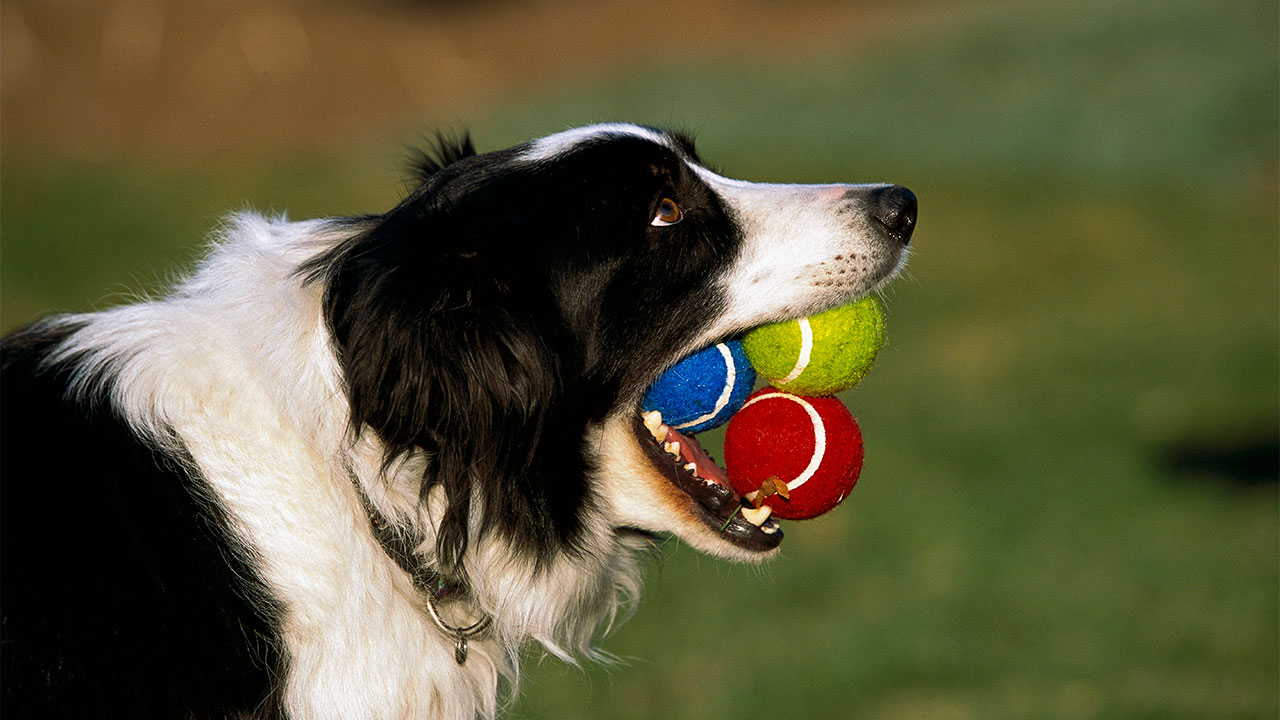
\includegraphics[scale=0.25]{./images/image.jpg}
		\caption{Исходное изображение}
	\end{figure}
	
	Её матрица не является квадратной (то есть имеем дело с общим случаем), и практически вся смысловая нагрузка приходится на левую часть изображения, а потому будет интересно проанализировать, что произойдёт с той же травой на заднем фоне.
	
	
	Итак, преобразуем нашу картинку к оттенкам черно-белого:
	\begin{figure}[h]
		\centering
		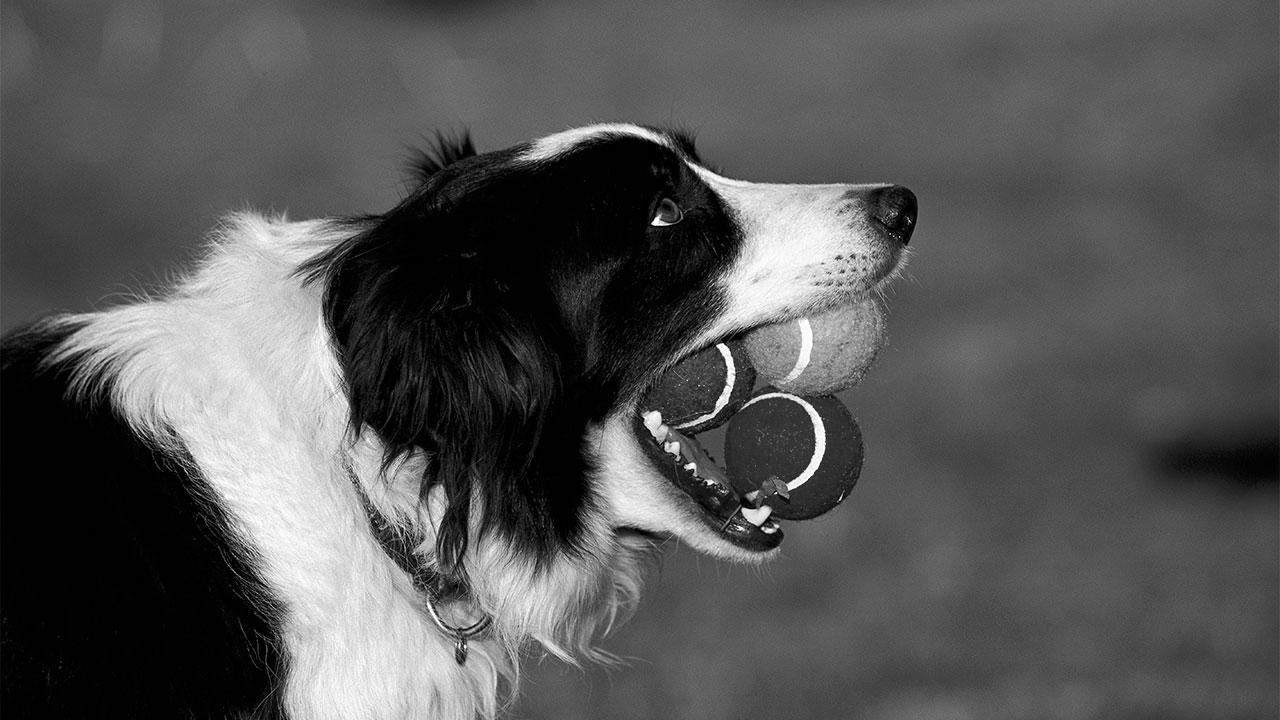
\includegraphics[scale=0.25]{./images/updated_image.jpg}
		\caption{Чёрно-белое изображение}
	\end{figure}
	
	И представим в виде матрицы, с помощью следующего кода:
	\begin{lstlisting}
rgb = imread("image.jpg");
upd = rgb2gray(rgb);
upd = im2double(upd); 
	\end{lstlisting}
	
	В переменной upd и лежит наше grayscale изображение, с ним и будем продолжать дальнейшую работу.
	
	Ощуществим SVD-разложение:
	\begin{lstlisting}
[U,S,V] = svd(upd);
V = transpose(V);
	\end{lstlisting}
	
	И выделим главное, оставив только $k=100$ первых наибольших сингулярных чисел и соответствующие им вектора матриц $U$ и $V$:
	\begin{lstlisting}
k = 100;
nu = U(:,1:k);
nv = V(1:k,:);
ns = S(1:k,1:k);
nimage = nu*ns*nv; % cutted image
	\end{lstlisting}
	
	На выходе получаем приемлемое качество картинки:
	\begin{figure}[h]
		\centering
		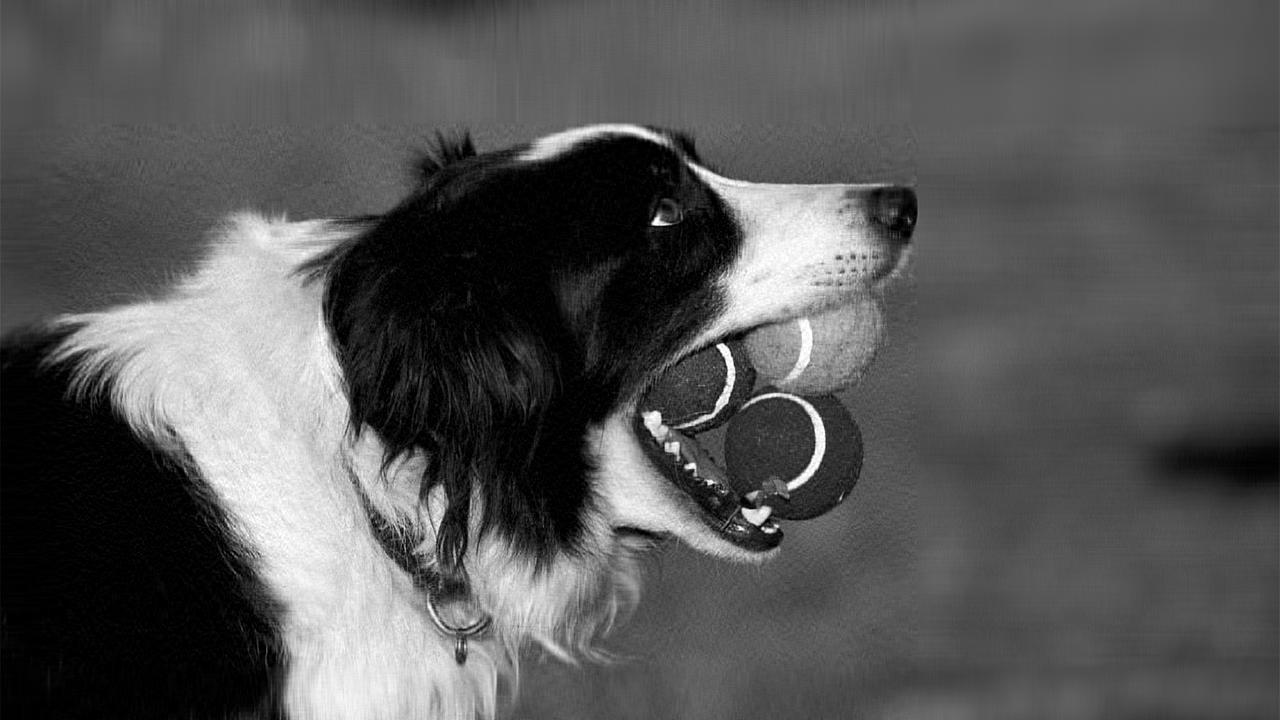
\includegraphics[scale=0.25]{./images/nimage100.jpg}
		\caption{Cжатое изображение при $k=100$, выгода в хранении - 0.2171}
	\end{figure}
	
	Видим, что задний фон картинки размыт, а собака как бы выделена из окружения различимым прямоугольником.
	
	Выгода в хранении задаёт отношение количества хранимых символов в обрезанном и исходном изображениях и, соответственно, вычисляется по формуле $\frac{mk + k + nk}{mn}$, где $m, n$ - количество строк и столбцов матрицы изображения.
	
	\subsection*{Различные ситуации}
	Проделаем ту же процедуру для различных значений $k$, вычисляя выгоду в хранении для каждого случая.
	
	\begin{figure}[h]
		\centering
		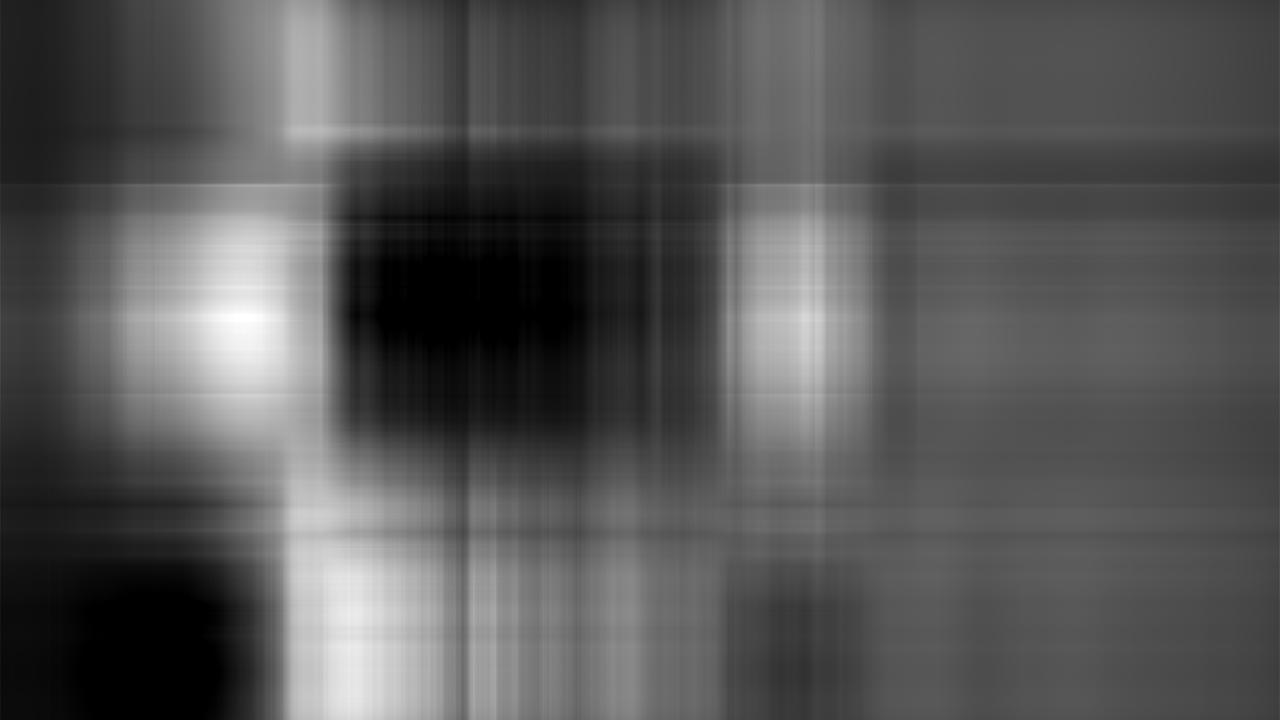
\includegraphics[scale=0.25]{./images/nimage2.jpg}
		\caption{Cжатое изображение при $k=2$, выгода в хранении - 0.0043}
	\end{figure}
	
	\begin{figure}[h]
		\centering
		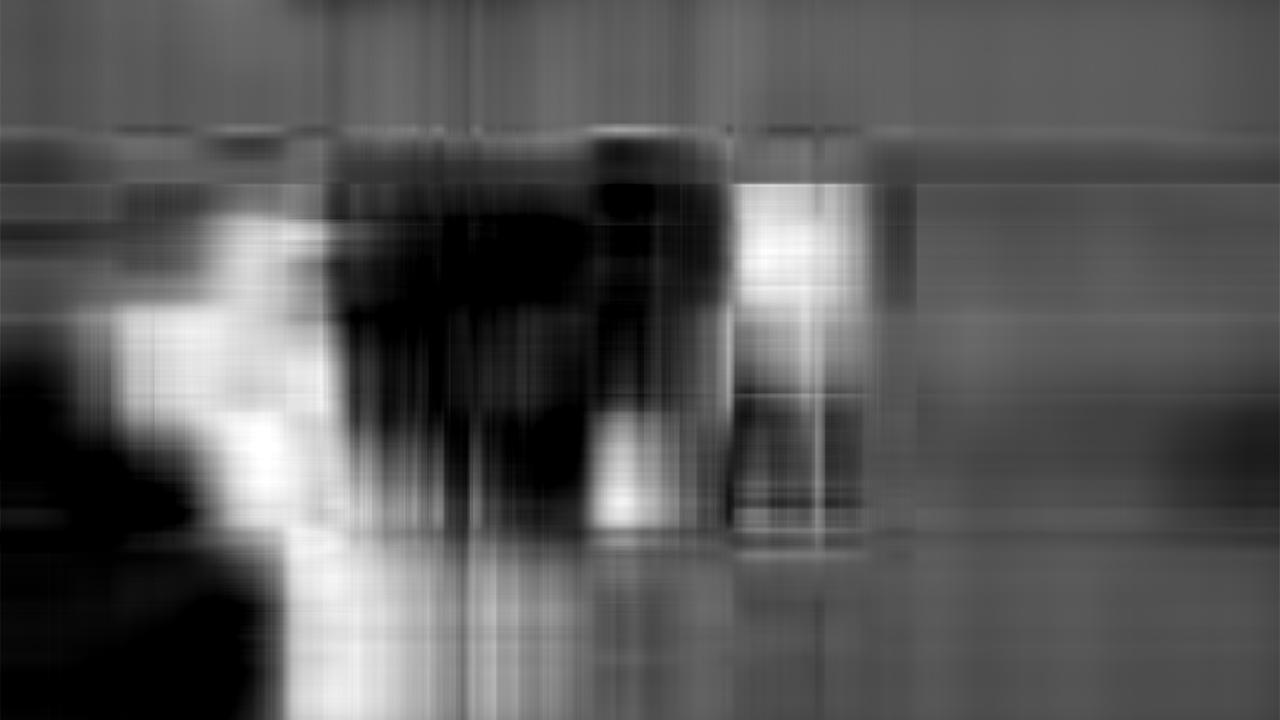
\includegraphics[scale=0.25]{./images/nimage5.jpg}
		\caption{Cжатое изображение при $k=5$, выгода в хранении - 0.0109}
	\end{figure}
	
	\pagebreak
	
	\begin{figure}[h]
		\centering
		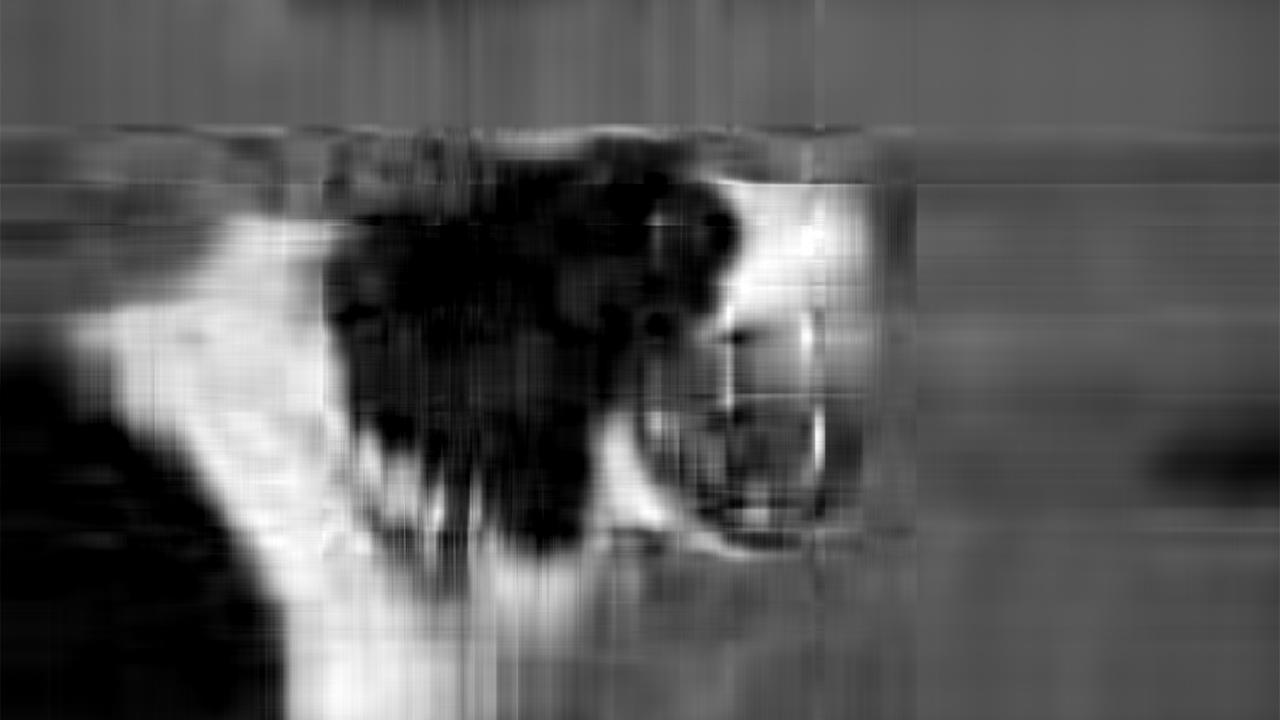
\includegraphics[scale=0.25]{./images/nimage10.jpg}
		\caption{Cжатое изображение при $k=10$, выгода в хранении - 0.0217}
	\end{figure}
	
	\begin{figure}[h]
		\centering
		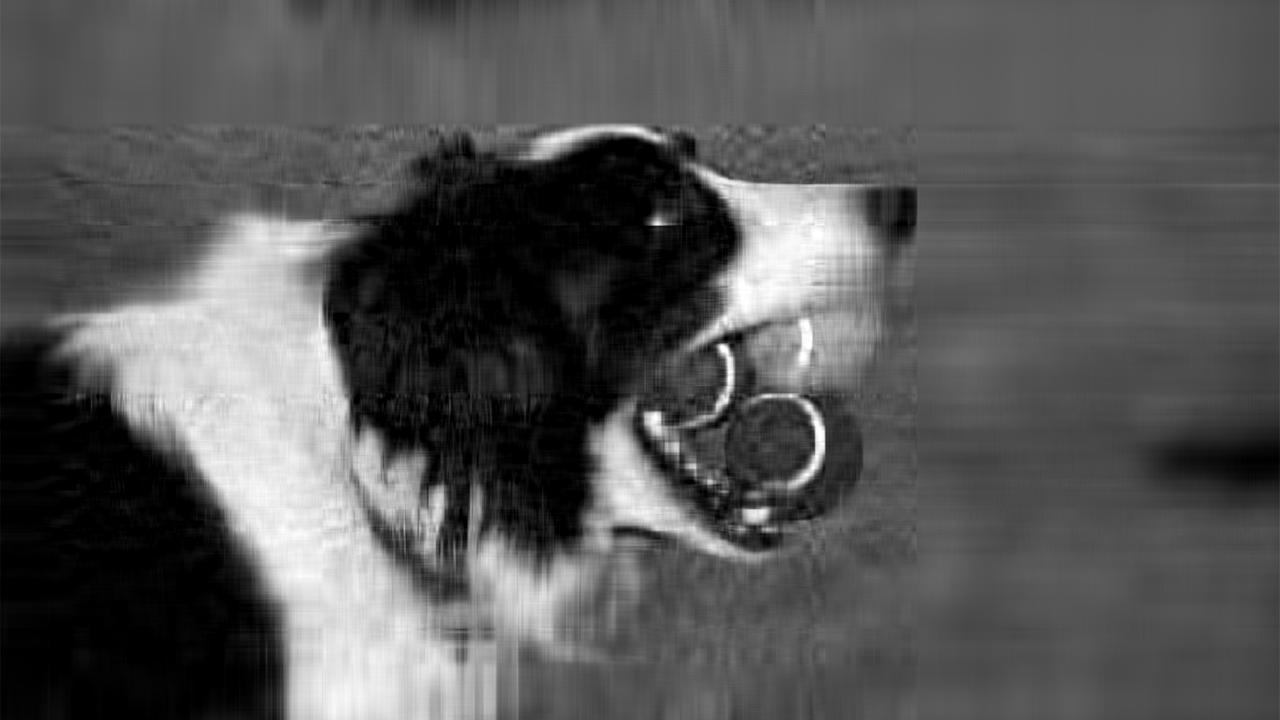
\includegraphics[scale=0.25]{./images/nimage25.jpg}
		\caption{Cжатое изображение при $k=25$, выгода в хранении - 0.0543}
	\end{figure}
	
	Видим, что при малых k картинка, как и ожидалось, превращается в неразличимую кашу, при $k=10$ уже можем различать какие-то детали и понять, что перед нами находится собака, а при $k=25$ картинка уже становится разборчивой и полностью доступной к пониманию.
	
	
	\begin{figure}
		\centering
		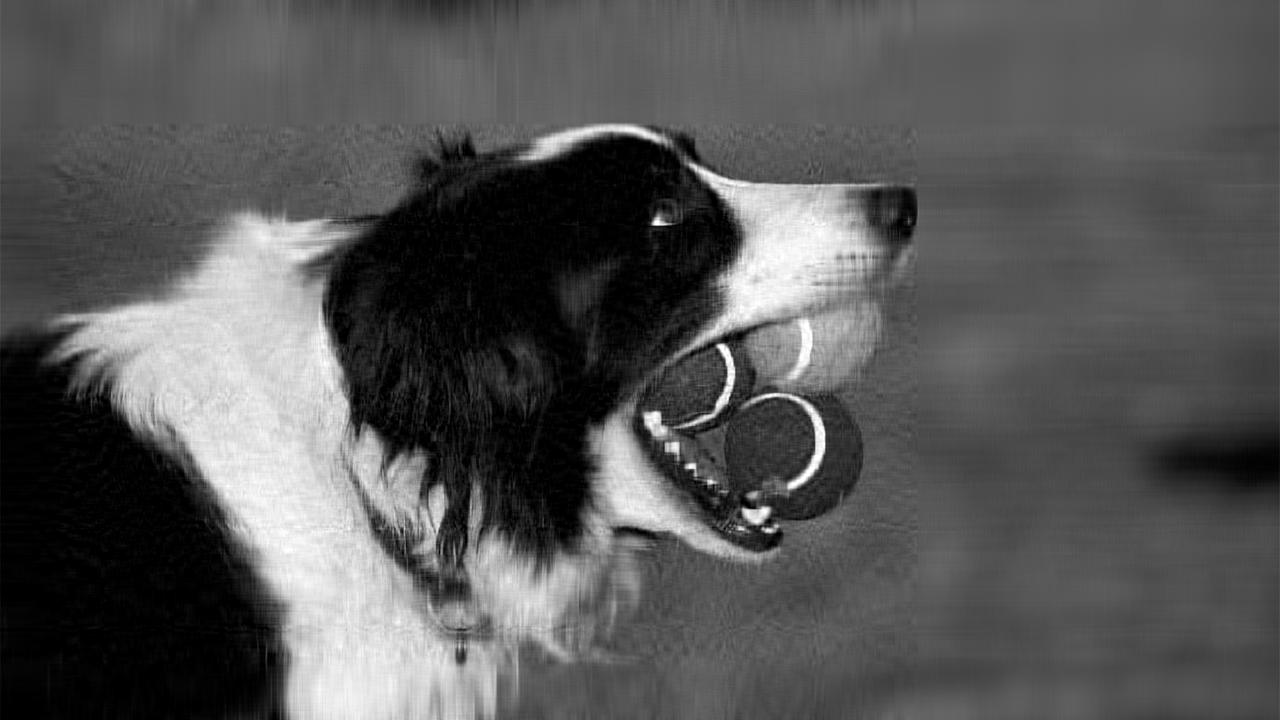
\includegraphics[scale=0.25]{./images/nimage50.jpg}
		\caption{Cжатое изображение при $k=50$, выгода в хранении - 0.1086}
	\end{figure}
	
	\begin{figure}
		\centering
		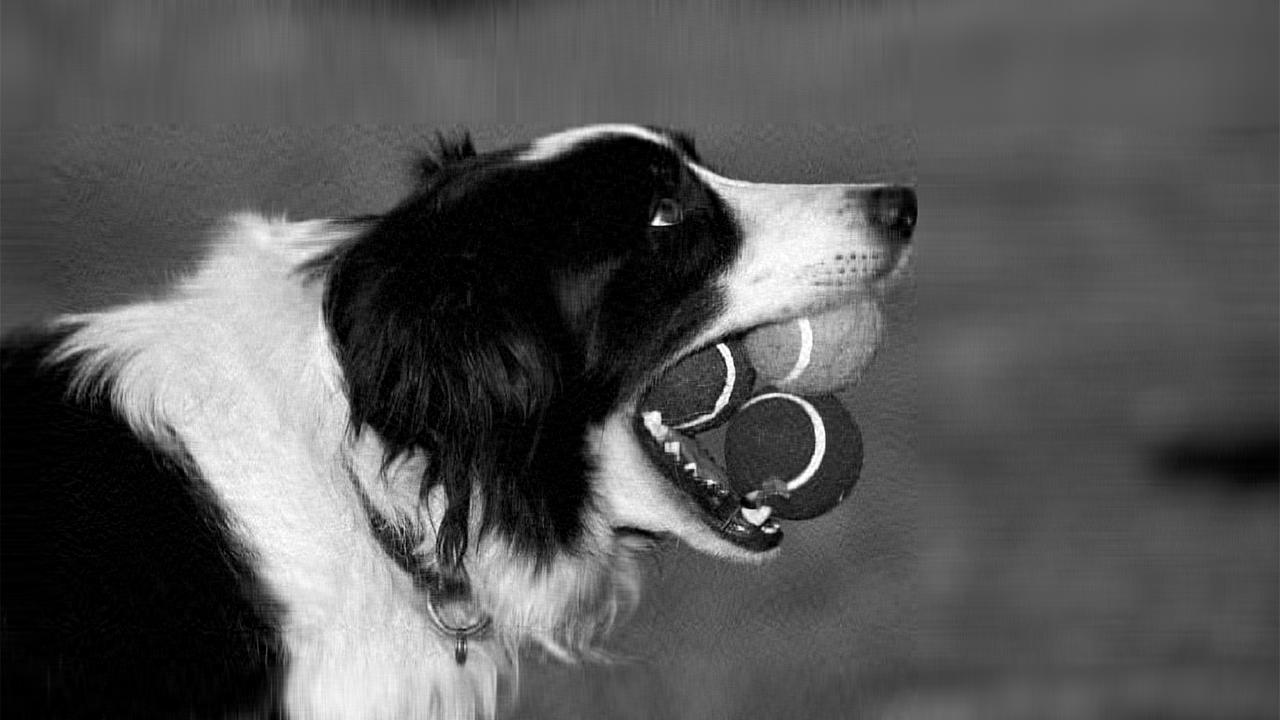
\includegraphics[scale=0.25]{./images/nimage75.jpg}
		\caption{Cжатое изображение при $k=75$, выгода в хранении - 0.1628}
	\end{figure}
	
	\pagebreak
	
	\begin{figure}[h]
		\centering
		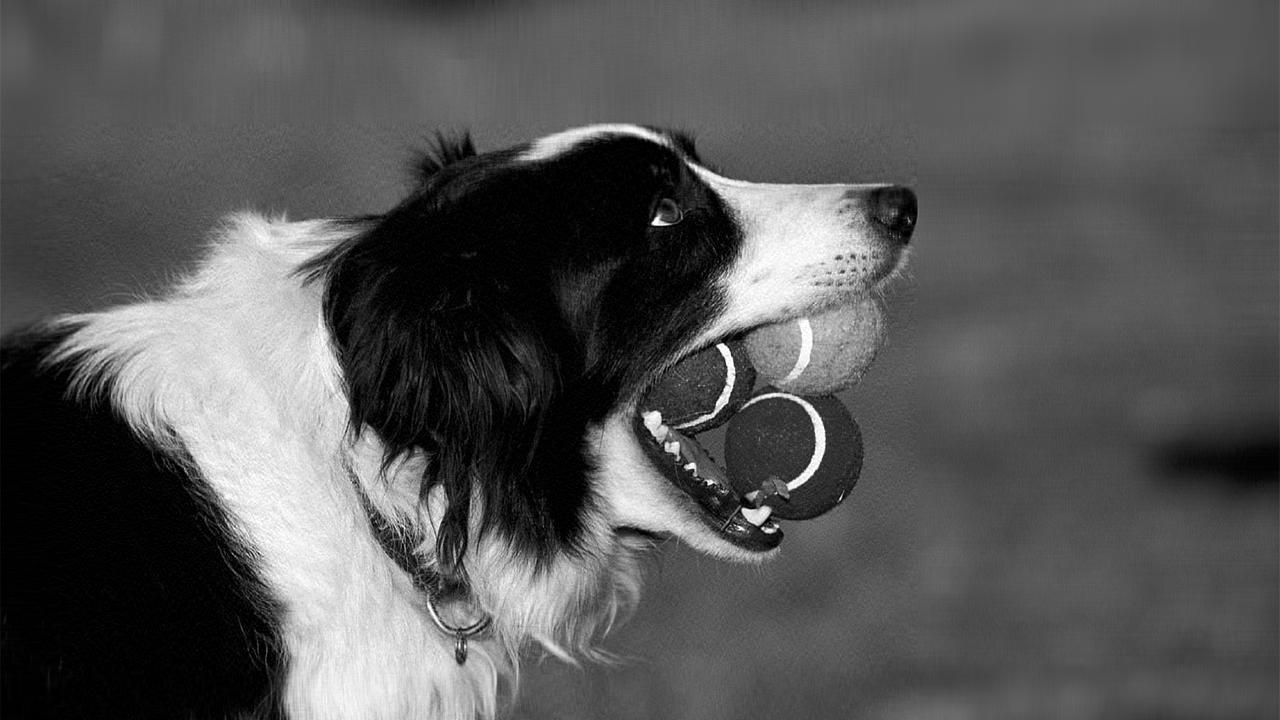
\includegraphics[scale=0.25]{./images/nimage150.jpg}
		\caption{Cжатое изображение при $k=150$, выгода в хранении - 0.3257}
	\end{figure}
	
	\begin{figure}[h]
		\centering
		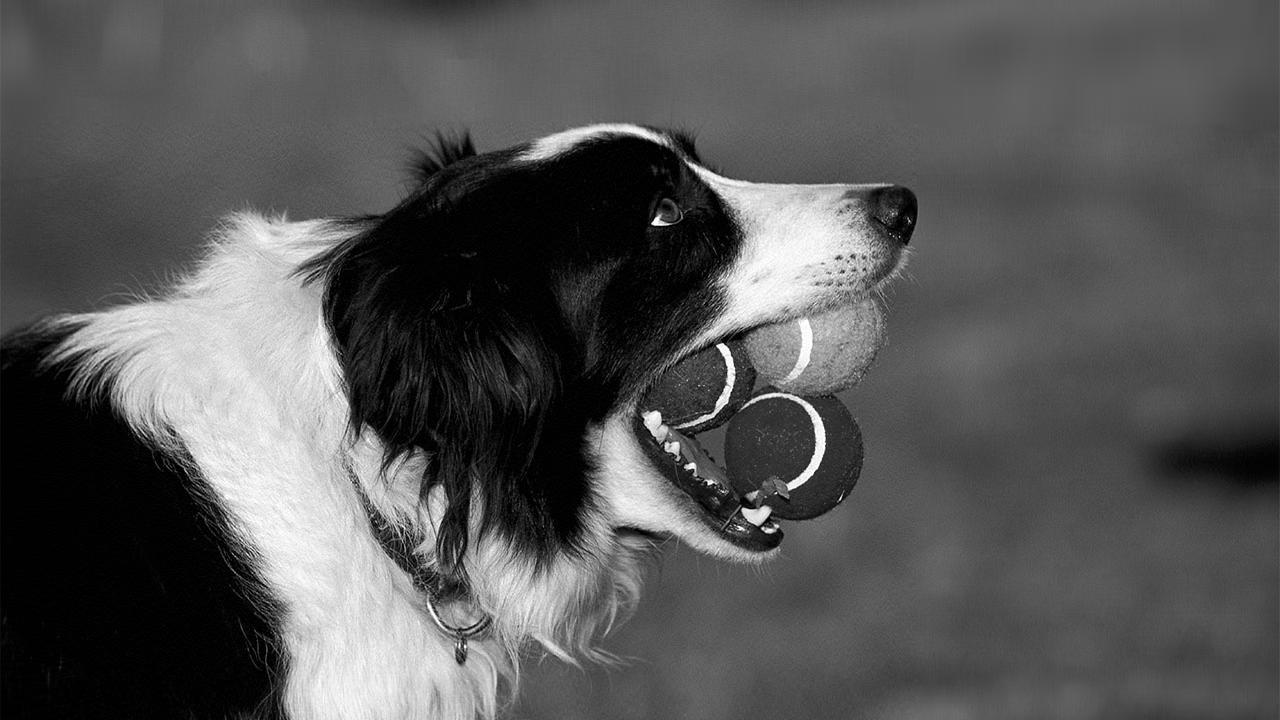
\includegraphics[scale=0.25]{./images/nimage250.jpg}
		\caption{Cжатое изображение при $k=250$, выгода в хранении - 0.5428}
	\end{figure}
	
	Можно заметить, что при $k=150$ и $k=250$ на картинках пропадает явно окружающий собаку прямоугольник, качество становится максимально приближенным к исходному.
	
	\pagebreak
	
	\begin{figure}[h]
		\centering
		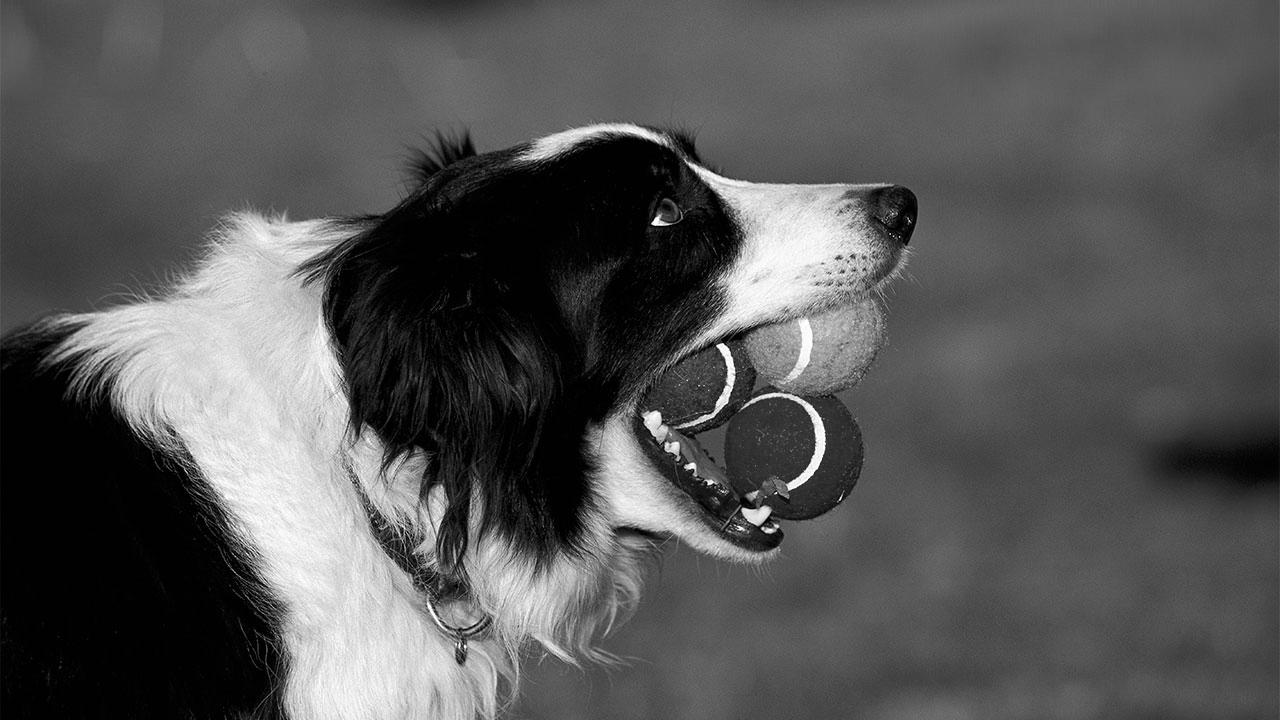
\includegraphics[scale=0.25]{./images/nimage500.jpg}
		\caption{Cжатое изображение при $k=500$, выгода в хранении - 1.0856}
	\end{figure}
	
	\begin{figure}[h]
		\centering
		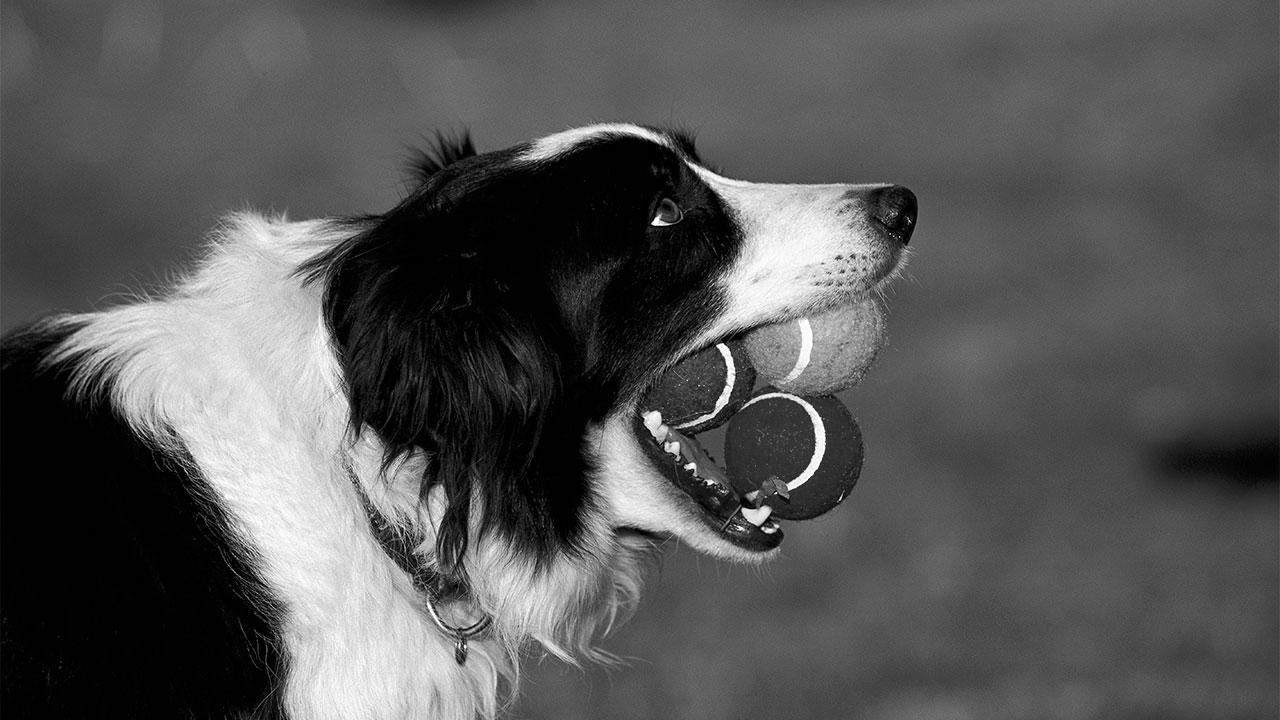
\includegraphics[scale=0.25]{./images/nimage700.jpg}
		\caption{Cжатое изображение при $k=700$, выгода в хранении - 1.5199}
	\end{figure}	
	
	
	На шаге $k=500$ хранить обрезанное изображение уже не имеет смысла, так как оно расходует больше памяти, чем исходное.
	
	Считаю, что наиболее сбалансированными является шаги $k=50$ и $75$, здесь мы получаем наилучшее соотношение качество/память. Если же мы хотим получить максимальное качество - идеальном будет $k=150$ и $250$.
	
	\textbf{На этом всё, спасибо!}
\end{document}